\section{Presentazione del modello di business}

Per la vendita del nostro prodotto puntiamo a rivolgerci direttamente al cliente finale, con alcune collaborazioni mirate insieme aziende già presenti nel settore. \\Per questo prevediamo la realizzazione di un \textit{e-commerce} per la vendita diretta al cliente e, in un primo periodo, la vendita anche su e-commerce già noti come \textit{Amazon} per avere un bacino di utenti più ampio. Sempre online, prevediamo di vendere il prodotto su alcuni e-commerce selezionati e specializzati nella vendita di piante e accessori per queste, così da raggiungere una clientela già interessata al mondo delle piante. Oltre alla vendita online, che crediamo sia quella per noi più importante, prevediamo di intraprendere delle partnership con aziende produttrici di vasi per la vendita di \textit{bundle vaso+PotNet}.

I costi di produzione stimati per singola unità, considerando solo i materiali, saranno compresi tra i 5 e gli 8 euro, con un prezzo di vendita ipotizzato tra i 25 e i 30 euro. \\Dopo alcuni mesi dalla commercializzazione del primo prodotto, prevediamo di commercializzare anche una versione di PotNet con un numero di sensori maggiore. Questo, a fronte di un costo di produzione di poco maggiore (2-3€), ci permetterà di vendere questa nuova versione ad un prezzo tra i 35 e i 40 euro, quindi con un utile superiore rispetto alla prima versione.

Oltre alla semplice vendita del prodotto, saranno presenti dei piani di abbonamento mensili a cui gli utenti potranno sottoscriversi per ottenere funzionalità aggiuntive sul bot Telegram e sulla Web UI. Prevediamo di lanciare questi abbonamenti ad un prezzo concorrenziale, tra 3 e 5 euro, in modo da convincere più clienti possibile a sottoscriversi andando così ad aumentare ancora di più la fidelizzazione del cliente verso l'azienda.

Crediamo quindi sia fondamentale puntare su una vendita prevalentemente online per raggiungere il nostro target di riferimento, il quale acquista principalmente su e-commerce.
Il nostro modello di business si basa quindi sui ricavi provenienti dalla vendita del prodotto e dalla sottoscrizione dei clienti agli abbonamenti aggiuntivi proposti. In questo modo uniamo il classico modello in cui la vendita del prodotto fisico rappresenta la maggior parte delle entrate, ad un modello in cui una funzionalità sviluppata una sola volta, continua a generare un profitto per vari mesi e/o anni.

\begin{figure}[ht!]
	\centering
	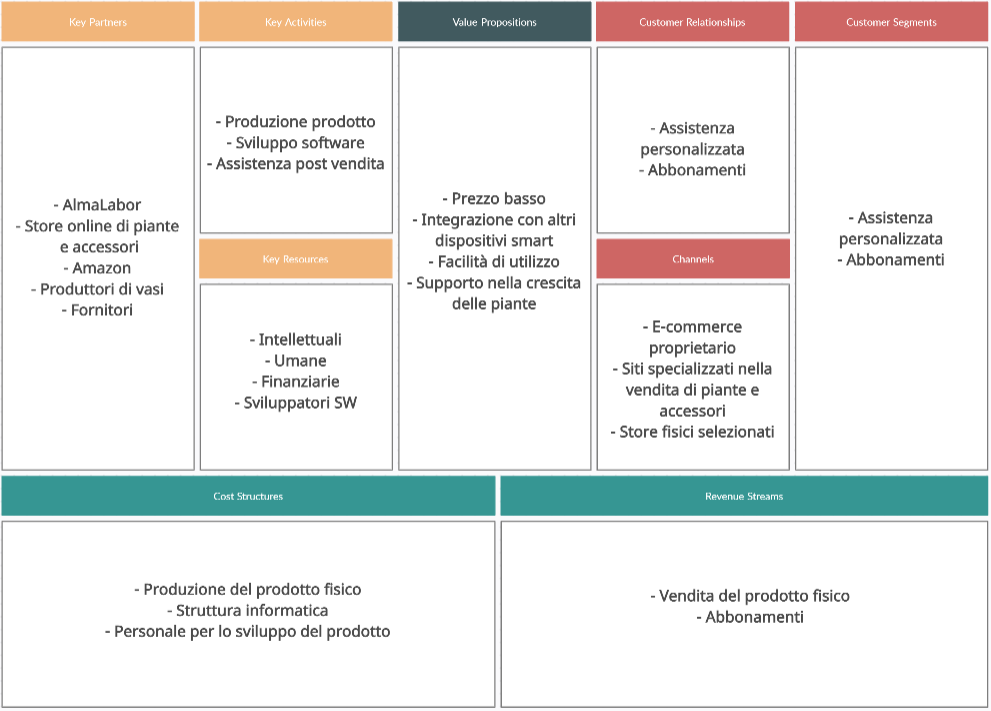
\includegraphics[width=\textwidth]{./images/Business-Model-Canvas.PNG} 
	\caption{Business Model Canvas \label{overflow}}
\end{figure}